\documentclass{homework}
% \usepackage{lua-visual-debug}
\usepackage{amsmath, amsfonts, amssymb}
\usepackage{enumitem}
\usepackage{graphicx}
% \usepackage[a4paper, total={6in, 8in}]{geometry}

\title{Midterm}
\subject{CS341 Introduction to Computer Networks}
\studentid{20170058}
\name{Keonwoo Kim}
\date{\today}

\setstretch{1.0}

\begin{document}
\maketitle

\parindent=0pt

{[1]} 1) \\
{[2]} 1), 2), 3) \\
{[3]} 1) \\
{[4]} 2) \\
{[5]} 1), 3) \\
{[6]} 2) \\
{[7]} 4) \\
{[8]} 2)


\subsection*{[Computer Networks in general]}

[1] Autonomous means that the system works as it is without any external interaction. For instance, a meeting with a closed room is an example of autonomous system.

[2] Protocols define how two different entity communicate. For instance, an application layer protocal defines four properties: the types of messages, the syntax and semantics of message fields and their alignments, and rules for sending and receiving the messages. Without protocols, computer devices cannot communicate each other due to lack of knowledges of how each other's messages are made.

[3] \begin{enumerate}[label={\arabic*)}]
    \item 5 users.
    \item 0.0729 (7.29\%)
\end{enumerate}

[4] [I'll assume the broken characters are $R$]
\begin{enumerate}[label={\arabic*)}]
    \item Assuming no other traffic in the network, the throughput for the file transfer is the minimum of the rates of links, which is $\min(R_1, R_2, R_3) = 200\,\text{kbps}$.
    \item $$\frac{2\,\text{MB}}{200\,\text{kbps}} = \frac{16\times 10^6 \,\text{bits}}{2\times 10^5\,\text{bps}} = 80\,\text{seconds}.$$
    \item The throughput is now $\min(R_1, R_2, R_3) = 500\,\text{kbps}$, and hence the transfer delay is roughly
    $$\frac{2\,\text{MB}}{500\,\text{kbps}} = \frac{16\times 10^6 \,\text{bits}}{5\times 10^5\,\text{bps}} = 32\,\text{seconds}.$$
\end{enumerate}

[5] Internet protocol stack is as follows:
Application layer (HTTP) / transport layer (TCP or UDP) / network layer (IP) / link layer (ethernet, WiFi, etc.) / physical layer (copper wire, optical fiber, etc.)\\
The Internet's architecture got its hourglass shape as every network communication in the Internet should pass through IP.

\subsection*{[Application layer]}

[1] The server differentiates the applications by the port numbers assigned to those applications.

[2] \begin{enumerate}
\item User's PC requests to the local DNS server.
\item If the local DNS server does not have any cache for the requested domain name ``google.com'', request to the `root server'.
\item The `root server' returns the IP address of the `.com server.'
\item The local DNS server requests to the `.com server.'
\item The `.com server' returns the IP address of the `google authoritative server.'
\item The local DNS server requests to the `.google authoritative server.'
\item The `.google authoritative server' resolves the `google.com' and tell the IP address of it to the local DNS server.
\item The local DNS server sends the IP address of the `google.com' to the user's PC.
\end{enumerate}

[3] No. the code \verb|s.recv(length-16)| may return a message with less than \texttt{length-16} bytes. Therefore, we need to repeatedly receive the pakcet from the socket \texttt{s} in order to ensure that the message is completely received.

[4] I think the problem is fairly broken.. No formulae are shown.
\begin{enumerate}[label={\arabic*)}]
  \item By visiting $n$ DNS servers, we need $n\cdot RTT$, and by requesting the page and the object, we need additional $8\cdot RTT$. So in total $(n+8)RTT$ is needed.
  \item By visiting $n$ DNS servers, we need $n\cdot RTT$, and by requesting the page and the object, we need additional $2\cdot RTT$ by using parallel connections. So in total $(n+2)RTT$ is needed.
  \item By visiting $n$ DNS servers, we need $n\cdot RTT$, and by requesting the page and the object, we need additional $RTT$ by using persistent connection. So in total $(n+1)RTT$ is needed.
\end{enumerate}

[5] Even if protocols provide various reliability, for instance, when a wrong message is received from the other, it may occur a panic. Thus, the end device should check the reliability once more.


\subsection*{[Transport Layer]}

[1] Suppose the message comes frequently from the other device. When we use NAK only, packet losses will be detected by missing sequence numbers quickly and corrupted packets will be detected by the NAK set by the other. So there is no problem. Also, by omitting ACK, we can get a performance gain. However, When the message comes infrequently, packet losses will not be detected until the we receive the next message. So we cannot differentiate between the packet loss and no message coming from the other device. It makes a problem. In summary, when the message comes frequently, NAK-only protocal have pros on performance; but when the message comes infrequently, NAK-only protocal have cons on reliability.


[2] 
1. Sender: Sends pkt0 and activate wait ACK0 state.\\
2. Receiver: Receives pkt0, sends ACK0 (with checksum), and activate `wait for 1 from below' state.\\
3. Sender: Receives ACK0, sends pkt1, and activate wait ACK1 state.\\
4. Receiver: Receives pkt1, sends ACK1 (with checksum), and activate `wait for 0 from below' state. But ACK1 is delayed.\\
5. Sender: Did not receive ACK1 and timed out, so resend pkt1 and remain in wait ACK1 state.\\
6. Receiver: receives pkt1 so resend ACK1 and remain in `wait for 0 from below' state.
5. Sender: receives ACK1 and this solves the problem.


[3]
\begin{enumerate}[label={\arabic*)}]
  \item Go-Back-N: when the sender did not receive the ACK for a packet and it timed out, the sender resends all the packets in the window from the oldest non-acknowledged packet. It may retransmit an acknowledged packet. When the bits in sequence numbers are $k$, the maximum window size is $2^k-1$. \\
  Selective Repeat: the sender only resends non-acknowledged packets in the window when the sender did not receive the ACK. It avoids unnecessary resending. When the bits in sequence numbers are $k$, the maximum window size is $2^{k-1}$. 
  \item a. GBN: packets $W/2, W/2+1,\cdots, 3W/2-1$ will be retransmitted;\\
  SR: packet $W/2$ will be retransmitted.\\
  b. GBN: At the time $t=T\cdot W/2$, the timer for packet $W/2$ starts. After the timeout of that timer, i.e., at $t=T\cdot W/2 + TO$, packets $W/2,\dots,W-1$ will be retransmitted. The transmission delay is $T\cdot W/2$ and the propagation delay will be $RTT/2$. Thus, in total, we need a time of $T\cdot W + TO + RTT/2$. \\
  SR: At the time $t=T\cdot W/2$, the timer for packet $W/2$ starts. After the timeout of that timer, i.e., at $t=T\cdot W/2 + TO$, packet $W/2$ will be retransmitted. The transmission delay is $T$ and the propagation delay will be $RTT/2$. Thus, in total, we need a time of $T\cdot (W/2+1)+ TO + RTT/2$. \\
  c. SR, since it has smaller delay when a single packet is lost.
\end{enumerate}

[4] 
\begin{enumerate}[label={\arabic*)}]
  \item 1 to 6, 23 to 26.
  \item 6 to 16, 17 to 22.
  \item A triple duplicate ACK.
  \item A timeout.
  \item 24.
  \item 12.
  \item At 6th transmission round.
\end{enumerate}

[5] Enough thoughput and enough burst tolerance for long flows, short delay enough for short flows.

\subsection*{[Discussion \& Suggestion]}

Question 4 in application layer section seems corrupted.

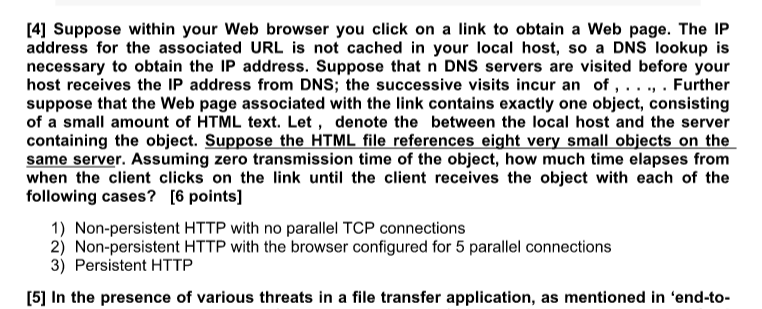
\includegraphics[width=\textwidth]{sc}

Thanks for your nice lectures.

\end{document}

